% questions.tex —— 1977 年·新疆卷（理科） · 题目内容片段（无答案）
% 由 tools/generate_projects.py 依来源总账自 1977/1977_数学真题_新疆理_试题.md 生成，勿手改（改源 MD 后重跑）


\gkpart{数学试题解（理工科）}

\begin{gktip}
\textbf{来源说明}：本题面依据固定源 PDF《新疆 1977 年高考数学试题解（理工科）》第 1—4 页逐题转录，解答依据同一 PDF 第 1—4 页核对。固定源是题面与解答连续出现的扫描材料，而不是无答案试卷；扫描件带书籍页码 125—127，第 4 页未见页码。原卷大题以「一」至「六」编号、参考题以「一」至「四」编号，本库按规范重排为第 1—6 题与参考题 1—4；「一」「三」之下的小题相应重排为连续小问（1）（2）……，未增删任何题干内容。
\end{gktip}

\begin{question}
\gkti{1}\textbf{（每小题 6 分）} 

（1） $\operatorname{Log}_3\dfrac{1}{27}=$\mbox{（　　）}；$\operatorname{Log}_{10}(\operatorname{Log}_{10}10)=$\mbox{（　　）}

（2） 当 $a$ 取什么值时，方程 $x^2-2x+\operatorname{Lg}a=0$ 有实数根。

\Needspace{5\baselineskip}
（3） 解方程：

\nopagebreak[4]
\[
7^{2x^2+x-6}=1.
\]

（4） 求等比数列 $\sqrt[6]{3}$，$\sqrt[3]{3}$，$\sqrt{3}$，…… 的公比 $q$，并写出它的第六项 $a_6$。

\Needspace{0.4\textheight}
\end{question}
\begin{question}
\gkti{2}\textbf{（16 分）} 在底边为 2 尺，高为 1.6 尺的三角形内截一个最大面积的矩形，并使其一边在三角形的底边上，求矩形的长和宽各是多少？
\nopagebreak[4]
\begin{center}% 1977 年新疆卷（理科）第二题：三角形 ABC 内截矩形 EFGH，一边 FG 在 BC 上，
% AD 为 BC 边上的高，K 为 AD 与 EH 的交点（按源卷第 2 页布局）
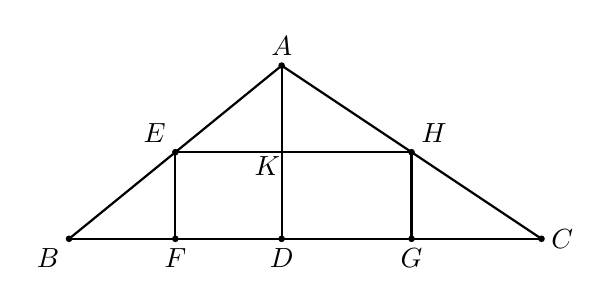
\begin{tikzpicture}[scale=1]
  \coordinate (B) at (0,0);
  \coordinate (C) at (6,0);
  \coordinate (A) at (2.7,2.2);
  \coordinate (D) at (2.7,0);
  \coordinate (E) at (1.35,1.1);
  \coordinate (H) at (4.35,1.1);
  \coordinate (F) at (1.35,0);
  \coordinate (G) at (4.35,0);
  \coordinate (K) at (2.7,1.1);
  \draw[thick] (B)--(C);
  \draw[thick] (A)--(B);
  \draw[thick] (A)--(C);
  \draw[thick] (A)--(D);
  \draw[thick] (E)--(H);
  \draw[thick] (E)--(F);
  \draw[thick] (H)--(G);
  \fill (A) circle (1.2pt) node[above] {$A$};
  \fill (B) circle (1.2pt) node[below left] {$B$};
  \fill (C) circle (1.2pt) node[right] {$C$};
  \fill (D) circle (1.2pt) node[below] {$D$};
  \fill (E) circle (1.2pt) node[above left] {$E$};
  \fill (F) circle (1.2pt) node[below] {$F$};
  \fill (G) circle (1.2pt) node[below] {$G$};
  \fill (H) circle (1.2pt) node[above right] {$H$};
  \node at (2.52,0.92) {$K$};
\end{tikzpicture}
\end{center}
\nopagebreak[4]
\end{question}
\begin{question}
\gkti{3}

（1） 求 $\operatorname{ctg}(-1200^\circ)$ 的值。（6 分）

（2） 已知 $\sin\alpha=-\dfrac{12}{13}$，并且 $\pi<\alpha<\dfrac{3\pi}{2}$，求 $\cos\dfrac{\alpha}{2}$。

\end{question}
\begin{question}
\gkti{4}\textbf{（12 分）} 三角形的三边长分别是 4 cm，5 cm，$\sqrt{61}$ cm，求这个三角形内最大角的度数。

\end{question}
\begin{question}
\gkti{5}\textbf{（18 分）} 求经过园 $2x^2-20x+2y^2+18=0$ 上一点 $p(3,\ 2\sqrt3)$ 的切线方程。

\begin{gktip}
\textbf{源注}：原卷「圆」印作「园」（第六题「园弧」、参考题四「椭园」同），本文按原卷用字保留。
\end{gktip}

\Needspace{0.4\textheight}
\end{question}
\begin{question}
\gkti{6}\textbf{（14 分）} 园弧拱桥的拱坡跨径 $AB=16$ 米，主拱高为 2.5 米，计算 $\overset{\frown}{AB}$ 的半径是多少米？
\nopagebreak[4]
\begin{center}% 1977 年新疆卷（理科）第六题：圆弧拱桥，弦 AB 为跨径，C 为拱顶，
% CD⊥AB 为主拱高，CD 延长线过圆心 O，OB=R（按源卷第 3 页布局）
\begin{tikzpicture}[scale=0.72]
  \coordinate (A) at (0,0);
  \coordinate (B) at (8,0);
  \coordinate (C) at (4,1.25);
  \coordinate (D) at (4,0);
  \coordinate (O) at (4,-5.775);
  \draw[thick] (A) arc[start angle=124.68, end angle=55.32, radius=7.025];
  \draw[thick] (A)--(B);
  \draw[dashed,->] (C)--(O);
  \draw[dashed,->] (B)--(O);
  \fill (A) circle (1.2pt) node[below left] {$A$};
  \fill (B) circle (1.2pt) node[right] {$B$};
  \fill (C) circle (1.2pt) node[above left] {$C$};
  \fill (D) circle (1.2pt) node[below left] {$D$};
  \fill (O) circle (1.2pt) node[below] {$O$};
  \node[right] at (6,-2.89) {$R$};
\end{tikzpicture}
\end{center}
\nopagebreak[4]
\begin{gktip}
\textbf{参考题}
\end{gktip}

\Needspace{5\baselineskip}
\textbf{参考题 1．} 解方程：

\nopagebreak[4]
\[
\operatorname{Log}_{16-3x}(x-2)=\operatorname{Log}_8 2\sqrt2.
\]

\Needspace{5\baselineskip}
\textbf{参考题 2．} 已知 $0^\circ<x<45^\circ$，且有

\nopagebreak[4]
\[
\operatorname{Lg}\operatorname{tg}x-\operatorname{Lg}\sin x
=\operatorname{Lg}\cos x-\operatorname{Lg}\operatorname{ctg}x
+2\operatorname{Lg}3-\frac{3}{2}\operatorname{Lg}2,
\]

试求 $\sin x-\cos x$ 的值。

\textbf{参考题 3．} 应用导数，求过曲线 $x^2+y^2-8x-2y+12=0$ 上一点 $p(5,\ 3)$ 的切线方程。

\textbf{参考题 4．} 利用定积分，求椭园 $4x^2+25y^2=100$ 的面积。

\end{question}